\documentclass{article}

\usepackage[preprint]{neurips_2020}
\usepackage[utf8]{inputenc}
\usepackage[T1]{fontenc}
\usepackage{hyperref}
\usepackage{url}
\usepackage{booktabs}
\usepackage{amsmath}
\usepackage{amsfonts}
\usepackage{graphicx}
\usepackage{multirow}
\usepackage[table]{xcolor}

\definecolor{blue300}{HTML}{9FD2F5}

\newcommand{\keywords}[1]{\vspace{0.6em}\noindent\textbf{Keywords:} #1}

\newcommand{\flowbox}[2]{
\setlength{\fboxsep}{4pt}
\fbox{\begin{minipage}[t]{#1}
\vspace{0.25em}
#2
\vspace{0.25em}
\end{minipage}}
}

\newcommand{\refcard}[3]{
\begin{minipage}[t]{0.23\textwidth}
\centering
\includegraphics[height=0.72in]{#1}\\[-0.15em]
{\scriptsize \textbf{#2}\\#3}
\end{minipage}
}

\newcommand{\resultcase}[4]{
\begin{minipage}[t]{0.30\textwidth}
\centering
\includegraphics[width=0.98\linewidth]{#1}\\[-0.2em]
{\scriptsize \textbf{#2}\\#3\\\emph{#4}}
\end{minipage}
}

\title{HearthGen for GraphML: LLM-Augmented Semantic Knowledge Graphs for Hearthstone Custom-Card Retrieval}

\author{
Yicheng Jin \quad Zhiheng Wang \quad Zicong Zhang\\
Rice University\\
\texttt{https://github.com/TraceOnSnow/HearthstoneCardGenerator}
}

\begin{document}

\maketitle

\begin{abstract}
Hearthstone custom-card design is a community-driven creative task in which users describe new cards through class identity, mechanics, stat lines, generated tokens, or references to existing cards. This makes the problem naturally graph-structured: cards connect to classes, types, keywords, actions, targets, resources, and derived-card relations. We present HearthGen as a GraphML project: an LLM-augmented semantic knowledge graph for retrieving mechanically relevant Hearthstone cards from natural-language custom-card requests. The system converts official card data into structured semantics, constructs a bipartite-style card--attribute graph, parses user requests into graph queries, and compares graph-based retrieval against TF-IDF, CLIP, and Node2Vec baselines. We also evaluate graph representation learning through held-out edge prediction. On 19 community-style DIY prompts, interpretable semantic KG retrieval achieves the best overall relevance@5 score (0.806), outperforming TF-IDF (0.679), CLIP (0.456), and Node2Vec graph embeddings (0.700). Node2Vec still learns useful graph structure, achieving 0.839 ROC-AUC and 0.858 average precision on held-out card-attribute edge prediction. These results show that Hearthstone card retrieval benefits from explicit semantic graph structure, while learned graph embeddings provide a complementary GraphML baseline.
\end{abstract}

\keywords{knowledge graphs, graph machine learning, retrieval-augmented generation, large language models, Node2Vec, game content generation}

\section{Introduction}

Hearthstone custom-card design is popular in online communities where players create new cards, discuss balance, and generate artwork for their ideas. A user may provide a vague request such as ``make a defensive Warrior card,'' a mechanic-first request such as ``a spell that freezes enemy minions,'' or a nearly complete card text that only needs artwork. The task is not simply text-to-image generation. A useful system must understand class identity, card type, mechanics, keywords, generated tokens, and references to existing card families.

This project studies the problem as a graph machine learning and LLM-graph synergy task. Hearthstone cards are naturally graph-structured: each card connects to semantic attributes such as class, type, keyword, action, target, resource, spell school, generated cards, and related cards. Instead of treating a card as unstructured text, we build a semantic knowledge graph (KG) where card nodes connect to typed attribute nodes. Natural-language custom-card requests are parsed into the same attribute space, allowing graph retrieval to match gameplay semantics.

A motivating example is the Hearthstone ``Rager'' meme. Magma Rager is a classic 3-mana 5/1 minion, and later cards with names such as Ice Rager and Faceless Rager continued the high-attack, low-health joke. If a user asks for ``a defensive Control Warrior Rager,'' the system must combine several signals: the Rager family reference, the 5/1 statline convention, and Warrior armor mechanics. Pure text retrieval can overfocus on keywords, and CLIP retrieval can return visually plausible but mechanically irrelevant images. A semantic graph can explicitly connect the request to both Rager-family anchors and Warrior armor cards.

Our contributions are:
\begin{itemize}
\item We construct a semantic Hearthstone KG from all card records, including collectible and derived cards.
\item We combine rule-based extraction and LLM enrichment to create structured card semantics and natural-language query parses.
\item We evaluate four retrieval methods: TF-IDF, CLIP, interpretable semantic KG matching, and Node2Vec graph embedding retrieval.
\item We evaluate GraphML structure learning through held-out card-attribute edge prediction.
\item We show a downstream application in KG-augmented card design and artwork generation.
\end{itemize}

\begin{figure*}[t]
\centering
\scriptsize
\setlength{\tabcolsep}{2pt}
\renewcommand{\arraystretch}{1.12}
\begin{tabular}{p{0.47\textwidth}p{0.47\textwidth}}
\rowcolor{blue300}
\multicolumn{2}{c}{\textbf{From natural language to graph retrieval and card generation}}\\[0.25em]
\flowbox{0.45\textwidth}{
\textbf{Natural-language request}\\
``DIY a new Rager meme card inspired by Magma Rager's 3-mana 5/1 statline, but make it a defensive Control Warrior card that gains Armor.''
}
&
\flowbox{0.45\textwidth}{
\textbf{Structured graph query}\\
class: Warrior; type: Minion; action: gain\_armor; related cards: Magma Rager, Rager; constraints: 5/1 statline, defensive Control Warrior, simple meme card.
}
\\[0.75em]
\rowcolor{blue300}
\multicolumn{2}{c}{\textbf{Faceted KG evidence: family anchor + mechanic anchor + class identity}}\\[0.25em]
\multicolumn{2}{c}{
\refcard{figures/figure1/magma_rager.jpg}{Magma Rager}{family/statline anchor}
\hfill
\refcard{figures/figure1/hookfist_3000.jpg}{Hookfist-3000}{Warrior armor mechanic}
\hfill
\refcard{figures/figure1/armorsmith.jpg}{Armorsmith}{class identity}
\hfill
\refcard{figures/figure1/eternium_rover.jpg}{Eternium Rover}{defensive flavor}
}
\\[0.75em]
\rowcolor{blue300}
\multicolumn{2}{c}{\textbf{Card design and generation prompt}}\\[0.25em]
\flowbox{0.45\textwidth}{
\textbf{Generated card text}\\
\textit{Iron Rager}. 3 Mana Warrior Minion, 5/1.\\
Battlecry: Gain 3 Armor.\\
Flavor: Molten fury tempered by iron will.
}
&
\flowbox{0.45\textwidth}{
\textbf{LoRA caption}\\
Hearthstone card art, a burly elemental rager forged from molten rock and clad in iron armor, Warrior class, glowing embers and metallic plates.
}
\\[0.75em]
\rowcolor{blue300}
\multicolumn{2}{c}{\textbf{Generated artwork and final playable-card composition}}\\[0.25em]
\begin{minipage}[t]{0.47\textwidth}
\centering
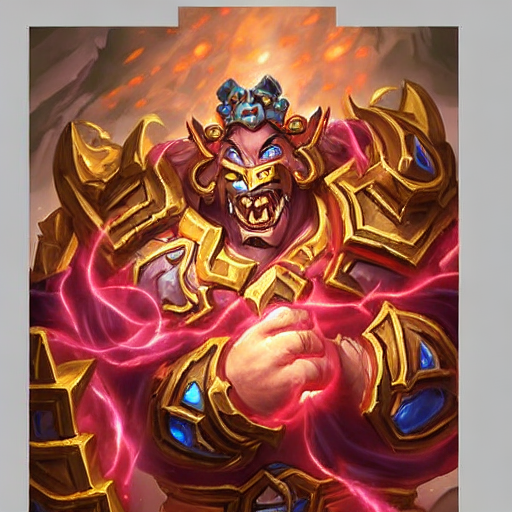
\includegraphics[height=1.15in]{figures/figure1/iron_rager_generated.png}\\[-0.2em]
{\scriptsize LoRA + KG reference output}
\end{minipage}
&
\begin{minipage}[t]{0.47\textwidth}
\centering
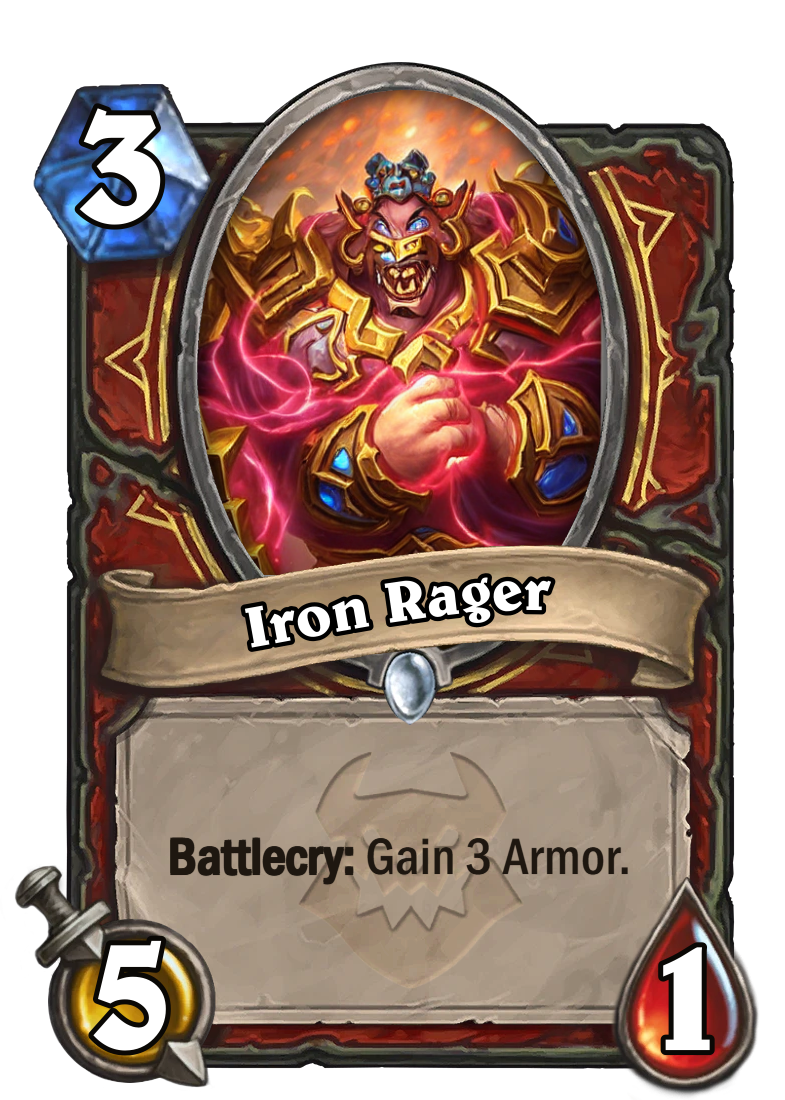
\includegraphics[height=1.15in]{figures/figure1/iron_rager_real_card.png}\\[-0.2em]
{\scriptsize External HearthDIY composition}
\end{minipage}
\end{tabular}
\caption{\textbf{End-to-end HearthGen case study.} A vague community-style request is parsed into graph attributes, matched against faceted KG evidence, converted into a playable card design and LoRA caption, and rendered as Hearthstone-style artwork. For the 559 project, the central technical object is the semantic graph and retrieval over it; image generation demonstrates the complete application.}
\label{fig:overview}
\end{figure*}

\section{Related Work}

\textbf{Graph representation learning.} Random-walk graph embeddings such as DeepWalk and Node2Vec learn node representations by treating sampled graph walks as sentences~\citep{perozzi2014deepwalk,grover2016node2vec}. Graph neural networks such as GCN and GraphSAGE instead propagate features over graph neighborhoods~\citep{kipf2017gcn,hamilton2017graphsage}. Our graph is heterogeneous and close to bipartite: cards connect to typed semantic attributes. We use Node2Vec because it is simple, scalable, and appropriate as a baseline for whether learned graph embeddings capture useful card-attribute structure.

\textbf{Retrieval-augmented generation.} Retrieval-augmented generation conditions downstream generation on external evidence~\citep{lewis2020rag}. Here, retrieval evidence is not free-form documents but structured card nodes and artwork references. This makes the retrieval stage interpretable: a result can be justified by shared class, type, action, keyword, or related-card nodes.

\textbf{Multimodal baselines.} CLIP maps text and images into a shared embedding space and is commonly used for text-to-image retrieval~\citep{radford2021clip}. CLIP is a strong visual baseline, but it does not explicitly encode gameplay mechanics. Our experiments compare CLIP retrieval with graph-based retrieval to test whether semantic graph structure adds value beyond visual similarity.

\textbf{Game content and image generation.} We use Stable Diffusion as a downstream image generator~\citep{rombach2022ldm} and a LoRA adapter for Hearthstone style adaptation~\citep{hu2021lora}. These components are not the main GraphML contribution; they demonstrate that retrieved graph evidence can support a realistic creative pipeline.

\section{Data and Semantic Graph Construction}

\subsection{Card Data}

We use Hearthstone card data from HearthstoneJSON and HearthSim tooling~\citep{hearthstonejson,hearthsim}. The dataset contains 8,661 total cards after filtering Battlegrounds and special-mode cards from the main semantic pipeline, with 6,149 collectible cards that also have artwork references for retrieval and generation experiments. Each raw card includes metadata such as class ID, card type ID, rarity, mana cost, attack, health, card text, keywords, and child card IDs.

\subsection{Structured Semantics}

We first convert raw card records into structured semantic records. Deterministic metadata fields are mapped directly from IDs to names: class, card type, set, rarity, spell school, minion type, mana cost, attack, health, durability, and keywords. Rule-based extractors identify common gameplay actions from card text, including \texttt{deal\_damage}, \texttt{summon}, \texttt{draw}, \texttt{gain\_armor}, \texttt{heal}, \texttt{freeze}, and \texttt{destroy}. LLM enrichment using MiniMax-M2.7 is used only for fields that rules often miss, such as implicit related-card references, generated-card roles, and concise semantic summaries~\citep{minimaxm27}. This design keeps factual fields deterministic while allowing LLMs to enrich ambiguous card semantics.

\subsection{Semantic Knowledge Graph}

The semantic KG is close to a bipartite graph. One side contains card nodes; the other side contains typed semantic attribute nodes. Attribute node types include class, card type, keyword, action, target, resource, spell school, minion type, generated card name, related card name, trigger, and condition. Edges include \texttt{HAS\_CLASS}, \texttt{HAS\_CARD\_TYPE}, \texttt{HAS\_KEYWORD}, \texttt{PERFORMS\_ACTION}, \texttt{TARGETS}, \texttt{AFFECTS\_RESOURCE}, \texttt{GENERATES\_CARD}, and \texttt{HAS\_CHILD\_CARD}.

Formally, we write the graph as
\begin{equation}
G=(V_c \cup V_a, E),
\end{equation}
where $V_c$ is the set of card nodes and $V_a$ is the set of semantic attribute nodes. Each typed edge is represented as $(c,a,r)$, where $c \in V_c$, $a \in V_a$, and $r$ is the relation type. This representation is intentionally not a generic text graph: relation types preserve gameplay meaning, so matching \texttt{PERFORMS\_ACTION: gain\_armor} is different from matching a visually similar card or a nearby word.

\begin{figure}[t]
\centering
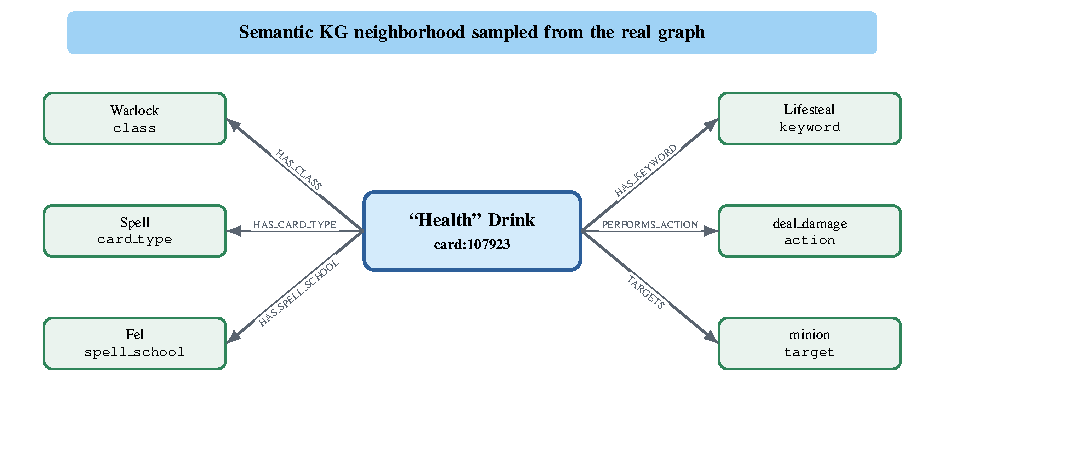
\includegraphics[width=\linewidth]{figures/kg/health_drink_kg_neighborhood.pdf}
\caption{\textbf{Semantic KG neighborhood sampled from the real graph.} The card node ``Health'' Drink connects to typed semantic attributes such as class, card type, spell school, keyword, action, and target. User queries are mapped into the same attribute space, allowing graph retrieval to match gameplay semantics.}
\label{fig:semantic_kg}
\end{figure}

\section{Methods}

\subsection{Natural-Language Query Parsing}

Each user request is converted into a structured query over KG attribute types. The query contains fields such as class, card type, actions, keywords, spell schools, generated card names, and related card names. We use deterministic pattern matching for common terms and LLM parsing when richer interpretation is needed. For example, ``defensive Control Warrior Rager'' maps to class \texttt{Warrior}, type \texttt{Minion}, action \texttt{gain\_armor}, and related card names \texttt{Rager} and \texttt{Magma Rager}.

The parsed query is a set of typed attribute constraints $A_q=\{(a,t)\}$ plus a short generated card description. This mirrors the examples supplied for the course: the system must define the graph object, the prediction/retrieval task, and the representation used by the graph model rather than only describing a software pipeline.

\subsection{Retrieval Methods}

We compare four retrieval methods.

\textbf{TF-IDF baseline.} We retrieve cards by lexical similarity over generated LoRA captions and semantic summaries. This baseline captures literal keyword overlap but does not use graph structure.

\textbf{CLIP baseline.} We retrieve card artworks by CLIP text-to-image similarity. This baseline tests whether visual embedding similarity alone can find useful references.

\textbf{Semantic KG matching.} We map query fields to KG attribute nodes and score each card by weighted neighborhood overlap. Actions and keywords receive higher weight than weak text overlap. This method is interpretable because each retrieved card includes matching graph reasons.

\textbf{Node2Vec graph embedding retrieval.} We train Node2Vec on the semantic KG. A query embedding is computed by averaging the embeddings of its matched attribute nodes, and cards are ranked by cosine similarity to this query embedding. This is the main learned GraphML retrieval baseline.

For explicit KG matching, the score is
\begin{equation}
s_{\mathrm{KG}}(c,q)=\sum_{a \in N(c) \cap A_q} w_{\tau(a)}+\lambda \cdot \mathrm{textOverlap}(c,q),
\end{equation}
where $\tau(a)$ is the attribute type and $w_{\tau(a)}$ gives higher weight to actions, keywords, class, and related-card nodes. For Node2Vec retrieval, let $z_v$ be the learned embedding of node $v$. We embed a query by averaging matched attribute embeddings:
\begin{equation}
z_q = \frac{1}{|A_q|}\sum_{a \in A_q} z_a,\qquad
s_{\mathrm{N2V}}(c,q)=\cos(z_c,z_q).
\end{equation}
This comparison separates two graph-based choices: symbolic typed-neighborhood matching versus learned random-walk embeddings.

\subsection{Held-Out Edge Prediction}

To test whether the graph representation captures reusable structure, we also run a link prediction experiment. We sample card-attribute edges, hold out 15\%, train Node2Vec on the remaining graph, and train a logistic regression classifier over edge features. Edge features concatenate the elementwise product and absolute difference of endpoint embeddings. We evaluate with ROC-AUC and average precision on balanced positive and negative test edges.

The link-prediction feature for a candidate edge $(u,v)$ is
\begin{equation}
\phi(u,v)=[z_u \odot z_v \, ; \, |z_u-z_v|],
\end{equation}
and the classifier estimates $p((u,v)\in E)=\sigma(\theta^\top\phi(u,v))$. This task evaluates whether graph embeddings can recover missing card--attribute facts, independently from the LLM query parser.

\section{Experiments}

\subsection{DIY Retrieval Evaluation}

We evaluate retrieval on 19 natural-language DIY prompts designed to reflect realistic custom-card use cases. The prompts include vague creative requests, mechanic-first requests, implicit related-card references, fully specified card text, and art-first requests. Each retrieval method returns top-5 cards. We evaluate class match, action match, relation match, and overall relevance using an LLM judge, then inspect qualitative cases manually.

For the GraphML run, Node2Vec uses 64 dimensions, walk length 12, 8 walks per node, window size 5, and random seed 13. The graph used for Node2Vec contains 6,149 card nodes and 68,223 typed card-attribute edges before filtering to the undirected embedding graph.

\begin{table}[t]
\centering
\small
\begin{tabular}{lcccc}
\toprule
\textbf{Method} & \textbf{Class@5} & \textbf{Action@5} & \textbf{Relation@5} & \textbf{Overall@5}\\
\midrule
TF-IDF & 0.7105 & 0.5337 & \textbf{0.7033} & 0.6788\\
CLIP & 0.4463 & 0.1258 & 0.5421 & 0.4557\\
Node2Vec & 0.7199 & 0.5535 & 0.6582 & 0.7002\\
Semantic KG & \textbf{0.8105} & \textbf{0.8145} & 0.6188 & \textbf{0.8061}\\
\bottomrule
\end{tabular}
\caption{\textbf{Retrieval relevance on 19 DIY prompts.} Semantic KG matching performs best overall because it directly matches typed gameplay attributes. Node2Vec improves over TF-IDF overall but is less precise than explicit KG matching for action semantics.}
\label{tab:retrieval}
\end{table}

\subsection{GraphML Edge Prediction}

The edge prediction task evaluates learned graph structure independently from the final retrieval pipeline. We sample 3,000 card-attribute edges, hold out 15\%, train Node2Vec on the remaining graph, and evaluate a logistic classifier on 900 balanced test edges.

Negative examples are sampled from card--attribute pairs that do not appear as KG edges. We keep the negative set balanced with positives so ROC-AUC and average precision measure ranking quality rather than majority-class behavior.

\begin{table}[t]
\centering
\small
\begin{tabular}{lrrrr}
\toprule
\textbf{Method} & \textbf{Train edges} & \textbf{Test edges} & \textbf{ROC-AUC} & \textbf{AP}\\
\midrule
Node2Vec + logistic regression & 5100 & 900 & 0.8389 & 0.8579\\
\bottomrule
\end{tabular}
\caption{\textbf{Held-out card-attribute edge prediction.} Node2Vec embeddings capture useful semantic graph structure, achieving strong ROC-AUC and average precision on unseen edges.}
\label{tab:link_prediction}
\end{table}

\subsection{Downstream Generation Evaluation}

Although the main 559 contribution is graph-based retrieval, we also evaluate and visualize the downstream image-generation application. We compare base Stable Diffusion 1.5 versus a Hearthstone LoRA adapter, and text-only versus reference-conditioned generation. The reference-conditioned setting uses retrieved Hearthstone artwork as visual evidence. Figure~\ref{fig:qualitative} shows the final LoRA + KG-reference outputs for six representative prompts.

\begin{figure*}[t]
\centering
\scriptsize
\setlength{\tabcolsep}{3pt}
\begin{tabular}{ccc}
\resultcase{figures/figure2/rager.png}{Iron Rager}{3 Mana Warrior Minion, 5/1. Battlecry: Gain 3 Armor.}{Vague meme/family request}
&
\resultcase{figures/figure2/druid_eclipse.png}{Eclipse Weaver}{4 Mana Druid Minion, 3/5. Battlecry: Add Solar Eclipse and Lunar Eclipse to your hand.}{Implicit related-card request}
&
\resultcase{figures/figure2/paladin_recruits.png}{Silver Hand Commander}{5 Mana Paladin Minion, 4/5. Battlecry: Summon two 1/1 Silver Hand Recruits.}{Token/archetype request}
\\[0.9em]
\resultcase{figures/figure2/mage_freeze.png}{Frozen Tempest}{5 Mana Mage Spell. Deal 2 damage to all enemy minions. Freeze them.}{Mechanic-first request}
&
\resultcase{figures/figure2/warrior_weapon.png}{Iron Oathbreaker}{3 Mana Warrior Weapon, 3/2. After your hero gains Armor, this weapon has +1 Attack.}{Fully specified card}
&
\resultcase{figures/figure2/bronze_dragon.png}{Chrono-Bronze Drake}{6 Mana Neutral Dragon, 5/7. Battlecry: Discover a card. If you control a Mech, reduce its Cost.}{Art-first request}
\end{tabular}
\caption{\textbf{LoRA + KG-reference qualitative outputs.} Six representative user prompts are shown as final generated artwork with the corresponding card description. The set mixes vague creative requests, implicit Hearthstone references, mechanic-first briefs, fully specified card text, and art-first requests.}
\label{fig:qualitative}
\end{figure*}

\begin{table}[t]
\centering
\small
\begin{tabular}{lrrrr}
\toprule
\textbf{Method} & \textbf{Prompt Align.} & \textbf{HS Style} & \textbf{Ref. Sim.} & \textbf{Quality}\\
\midrule
SD text-only & 0.2958 & 0.7499 & -- & 0.4972\\
SD + reference & 0.2951 & 0.8366 & 0.7962 & 0.5024\\
LoRA text-only & \textbf{0.3013} & 0.8581 & -- & \textbf{0.5022}\\
LoRA + reference & 0.2968 & \textbf{0.8608} & \textbf{0.8303} & 0.5008\\
\bottomrule
\end{tabular}
\caption{\textbf{Downstream generation proxy metrics.} LoRA improves Hearthstone style, and reference conditioning increases similarity to retrieved card evidence. These image metrics are secondary to the GraphML evaluation.}
\label{tab:generation}
\end{table}

\section{Results and Discussion}

Table~\ref{tab:retrieval} shows that explicit semantic KG retrieval performs best overall. The largest gain is in action matching: 0.8145 for KG retrieval versus 0.5535 for Node2Vec, 0.5337 for TF-IDF, and 0.1258 for CLIP. This supports the main hypothesis of the project: Hearthstone custom-card requests are structured around gameplay semantics, and a typed card-attribute graph represents those semantics better than raw text or visual similarity alone.

Node2Vec is still useful. It improves overall retrieval over TF-IDF and CLIP, and Table~\ref{tab:link_prediction} shows that learned graph embeddings capture card-attribute structure well. However, learned embeddings blur some exact semantics. For example, graph proximity may retrieve cards in the same class or archetype but miss the specific requested action. In contrast, explicit KG matching can preserve hard constraints such as \texttt{PERFORMS\_ACTION = gain\_armor}. This is a useful finding for GraphML applications: learned graph embeddings are strong for structural generalization, while symbolic graph matching remains valuable when attributes are semantically typed and sparse.

CLIP performs worst for gameplay relevance. This is expected because CLIP sees visual and textual similarity, not Hearthstone rule structure. It can retrieve fantasy images that look plausible but fail to match class or mechanic. TF-IDF does better than CLIP for text-heavy prompts but over-relies on literal keywords and can miss implicit card relationships.

The Rager case illustrates why graph evidence is useful. A flat ranking may over-rank Warrior armor cards because they match class and action, while under-ranking Magma Rager because it does not match armor mechanics. For card design, both are needed: Magma Rager provides the family/statline anchor, while Warrior armor cards provide mechanic evidence. We therefore view KG retrieval not only as a top-k ranking problem but also as evidence construction over multiple semantic facets.

The downstream generation results in Table~\ref{tab:generation} are consistent with the retrieval story. LoRA improves style similarity, while reference conditioning makes the generated image closer to retrieved evidence. However, automatic image metrics are only proxy measures. The main technical contribution for this course is the graph representation and retrieval method, not the image model itself.

\section{Challenges and Limitations}

The first challenge was semantic extraction. Hearthstone card text contains implicit mechanics, generated tokens, and references to other cards. Pure rules cover common actions such as damage, healing, armor, and summoning, but LLM enrichment is needed for implicit relationships such as Solar Eclipse/Lunar Eclipse or Rager-family references.

The second challenge was evaluation. There is no standard benchmark for Hearthstone custom-card retrieval. We created 19 community-style prompts and used an LLM judge to score retrieval relevance. This is practical for a course project, but future work should include larger human evaluation.

The third challenge was balancing interpretability and learned GraphML. Node2Vec provides a clean graph embedding baseline and performs well on link prediction, but explicit KG matching is more interpretable and more accurate for exact mechanic retrieval. A stronger future system could combine both, for example by using KG rules for hard constraints and graph embeddings for soft semantic expansion.

\section{Student Contributions}

All team members contributed to project design and final analysis. Yicheng Jin focused on semantic representation design, KG construction, retrieval evaluation, report writing, and integration. Zhiheng Wang contributed to data processing, LoRA/diffusion experiments, generation evaluation, and final result preparation. Zicong Zhang contributed to baseline retrieval, experiment scripting, qualitative examples, and evaluation support.

\section{Conclusion}

HearthGen demonstrates a novel LLM-graph application for game-content generation. By converting Hearthstone cards into a semantic card-attribute graph, the system can retrieve mechanically relevant and interpretable evidence from natural-language custom-card requests. Explicit KG retrieval outperforms TF-IDF, CLIP, and Node2Vec retrieval on overall relevance, while Node2Vec achieves strong held-out edge prediction performance. These results suggest that structured game domains are a promising setting for combining LLMs, knowledge graphs, and graph representation learning.

\bibliographystyle{plainnat}
\bibliography{references}

\end{document}
